\documentclass[11pt]{beamer} %Add 'handout' in the options for printing

\usepackage{beamercolorthemewolverine}
\usetheme{AnnArbor}

\usepackage[english]{babel}
\usepackage{amsmath,amssymb}
\usepackage{mathtools}
\usepackage{commath}
\usepackage{amssymb,amscd,amsfonts,amsbsy}
\usepackage{enumerate}
\usepackage{epsfig}
\usepackage{pgfpages}
\usepackage{graphics}
\usepackage{graphicx}
\usepackage{multicol}
\usepackage{layouts}
\usepackage[center]{caption}
\usepackage{natbib}
%\usepackage{movie15}
\usepackage{etex}
\usepackage[export]{adjustbox}
\usepackage{embedfile}
\usepackage{caption}
\usepackage{soul,xcolor}
\usepackage{import}
\usepackage{relsize}
\usepackage{tikz}
\usepackage[makeroom]{cancel}
\usepackage{multimedia}
\usepackage{subcaption}
\usepackage{comment}
%\usepackage{media9}



%Setup note page
\setbeamertemplate{note page}[plain]
%\setbeameroption{show notes on second screen=right}
%\setbeameroption{show notes on second screen=left}

\setbeamertemplate{navigation symbols}{}%remove navigation symbols

\setbeamertemplate{footline}[frame number]{}%gets rid of bottom navigation bars


\graphicspath{ {../figs/lung_figs/} }


% Figures within a column...
\makeatletter
\newenvironment{tablehere}
{\def\@captype{table}}
{}
\newenvironment{figurehere}
{\def\@captype{figure}}
{}
\makeatother

\newcommand{\beginbackup}{
   \newcounter{framenumbervorappendix}
   \setcounter{framenumbervorappendix}{\value{framenumber}}
}
\newcommand{\backupend}{
   \addtocounter{framenumbervorappendix}{-\value{framenumber}}
   \addtocounter{framenumber}{\value{framenumbervorappendix}} 
}

%---------------------------------------------------------------------------
%\setbeamercolor{mycolor}{fg=White,bg=White}
\setbeamercolor{alerted text}{fg=red} 
\setbeamertemplate{frametitle}
{
  \vskip-5pt 
  \leavevmode
  \begin{center}
    \vspace*{-0.5cm}
  \hbox{%
  \begin{beamercolorbox}[wd=0.85\paperwidth,ht=0.35cm,dp=1.35ex]{White}%
    \raggedright
    \vspace*{-.25cm}
    {\normalsize \insertframetitle} %\small{\insertframetitle}
  \end{beamercolorbox}
  % \hspace*{1em}{\normalsize \insertframetitle} %\small{\insertframetitle}
  }%
  \end{center}
  \vspace*{-0.75cm}
}
\def\newblock{\hskip .11em plus .33em minus .07em}

\setbeamertemplate{headline}{}

\setbeamercovered{dynamic}


\newcommand{\RR}{{\mathbb{R}}}
\newcommand{\NN}{{\mathbb{N}}}
\newcommand{\ZZ}{{\mathbb{Z}}}
\newcommand{\CC}{{\mathbb{C}}}
\newcommand{\eps}{\varepsilon}
\newcommand{\bp}{\noindent {\it Proof}.\,\,\,}
\newcommand{\ep}{\hfill$\Box$ \vskip 0.08in}
\newcommand{\dint}{\int\!\!\!\int}
\newcommand{\vs}{\vskip 0.5cm}
\newcommand{\po}{{\partial\Omega}}
\newcommand{\meanint}{{\int{\mkern-19mu}-}}
\def\ring{\mathaccent"0017 }

\definecolor{AliceBlue}{RGB}{240,248,255}


%\definecolor{lightblue}{rgb}{1,0,0}
%\sethlcolor{lightblue}
\renewcommand<>{\hl}[1]{\only#2{\beameroriginal{\hl}}{#1}}

% http://tex.stackexchange.com/questions/41683/why-is-it-that-coloring-in-soul-in-beamer-is-not-visible
\makeatletter
\newcommand\SoulColor{%
  \let\set@color\beamerorig@set@color
  \let\reset@color\beamerorig@reset@color}
\makeatother
\SoulColor



%\usepackage{media9}%
%\newcommand{\includemovies}[3]{%
%\includemedia[%
%width=#1,height=#2,%
%activate=pagevisible,%
%deactivate=pageclose,%
%addresource=#3,%
%flashvars={%
%src=#3 % same path as in addresource!
%&autoPlay=true % default: false; if =true, automatically starts playback after activation (see option ‘activation)’
%&loop=true % if loop=true, media is played in a loop
%&controlBarAutoHideTimeout=0 %  time span before auto-hide
%}%
%]{}{StrobeMediaPlayback.swf}%
%}



%%% Local Variables:
%%% mode: latex
%%% TeX-master: "../main"
%%% End:

\embedfile{\jobname}
\embedfile{include/preamble.tex}
% 

% My commands
\newcommand{\orderof}[1]{\ensuremath{\mathcal{O}\left(#1\right)}}
\newcommand{\plus}{\raisebox{.2\height}{\scalebox{.8}{+}}}
\newcommand{\minus}{\raisebox{.2\height}{\scalebox{.8}{-}}}
\newcommand{\timesx}{\raisebox{.2\height}{\scalebox{.8}{\times}}}
\newcommand{\equals}{\raisebox{.25\height}{\scalebox{0.9}{=}}}
\renewcommand{\CancelColor}{\color{red}} %change cancel color to red

\makeatletter
\let\my@cancelto\cancelto %copy over the original cancelto command
\newcommand<>{\cancelto}[2]{\alt#3{\my@cancelto{#1}{#2}}{\mathrlap{#2}\phantom{\my@cancelto{#1}{#2}}}}
% redefine the cancelto command, using \phantom to assure that the
% result doesn't wiggle up and down with and without the arrow
\makeatother


\begin{document}
%% Some customizations, based on https://tex.stackexchange.com/questions/22346/how-to-customize-titlepage-in-beamer

% \defbeamertemplate*{title page}{customized}[1][]
% {
% %  \usebeamerfont{title}\inserttitle\par
% %  \usebeamerfont{subtitle}\usebeamercolor[fg]{subtitle}\insertsubtitle\par
% %  \bigskip
%  % \usebeamerfont{author}\insertauthor\par
% %  \usebeamerfont{institute}\insertinstitute\par
% %  \usebeamerfont{date}\insertdate\par
%   \usebeamercolor[fg]{titlegraphic}\inserttitlegraphic
% }


%%
\title[]{Applications of Computation in Acoustics:\\Ultrasound Bioeffects \&\\ Underwater Transmission Loss Uncertainty}
\author[] {}

\institute[]{}
\date[date]{}


\begin{frame} %\vspace{1cm}
  \vspace*{1cm}
  %\titlepage \vspace{-2.50cm}

  {
    %\definecolor{darkpowderblue}{rgb}{0.0, 0.2, 0.6} %% UNCOMMENT IF NOT IN PREAMPLE
    \setbeamercolor{title}{fg=white, bg=darkpowderblue}
  \begin{beamercolorbox}[sep=8pt,center,wd=\paperwidth,ht=0.3\textheight,dp=0.045\textheight]{title}
    \usebeamerfont{title}\inserttitle\par%
  \end{beamercolorbox}
  }
  \centering
  \begin{columns}
    \column{.25\textwidth}
    
    % \begin{figure}\vspace*{1.3cm} \centering 
\includegraphics[width=.70\columnwidth]{include/figs/MichiganSeal} \end{figure}
    \column{.5\textwidth}
    \begin{center}
      % 
      \normalsize{A \emph{dissertation defense} by:\\Brandon Patterson} \vspace{16pt} \\ 
      % 
      \footnotesize{Scientific Computing and Flow Physics Lab} \vspace{4pt}\\
      \footnotesize{University of Michigan, Ann Arbor} \vspace{4pt}\\
      \scriptsize{Department of Mechanical Engineering} \vspace{4pt}\\
      % \scriptsize{$^2$Department of Radiology} \vspace{4pt}
    \end{center}
    \column{.25\textwidth}
    \vspace*{.15cm}
    % \begin{figure} \vspace*{1.3cm} \centering 
\includegraphics[width=.70\columnwidth]{include/figs/MElogo} \end{figure}
  \end{columns}
  \vspace{.25cm}
  \begin{center}
    % 
    % 
    %%%%%%%%%%%%%%%%%%% Put Date Here   %%%%%%%%%%%%%%%%%%%%%%%%%%%%
    % \footnotesize {\today} \vspace{-.1cm}
    \footnotesize {October 31, 2017} \vspace{-.1cm}
    % 
    % 
  \end{center}



  % 
  % 
  %%%%%%%%%%%%%%%%%%% FUNDING SOURCE OR CONFERENCE IMAGES BELOW ( L | C | R )   %%%%%%%%%%%%%%%%%%%%
  \begin{minipage}{\textwidth}
    \hspace*{.5cm}
    \begin{minipage}{.3\textwidth}
      \begin{center} 
        \begin{figure}
          \centering
          % \includegraphics[width=.4\textwidth]{include/figs/NIH_logo}
          %	\label{fig:NIH_logo_blue}
        \end{figure}
      \end{center}
    \end{minipage}
    \begin{minipage}{.3\textwidth}
      \begin{center} 
        \begin{figure}
          \centering
          % \includegraphics[width=.8\textwidth]{include/figs/nsfgrfp}
          \label{fig:NSF_logo_blue}
        \end{figure}
      \end{center}
    \end{minipage}
    \begin{minipage}{.3\textwidth}
      \begin{center} 
        
      \end{center}
    \end{minipage}
  \end{minipage}
\end{frame}
%%% Local Variables:
%%% mode: latex
%%% TeX-master: "../main"
%%% End:




%%%%%%%%%%%%%%%%%%%%%%%%%%%%%%%% Slides %%%%%%%%%%%%%%%%%%%%%%%%%%%%%%
\begin{frame}
  \vfill
  \begin{figure}
    \centering
    \includegraphics[height=0.25\textheight]{./include/figs/CoE-ME-vert} \hfill
    \includegraphics[height=0.25\textheight]{./include/figs/mcubed_logo} \hfill
    \includegraphics[height=0.25\textheight]{./include/figs/NIH_logo_white}\hfill
  \end{figure}
  \vfill
  \begin{figure}
    \centering
    \includegraphics[height=0.25\textheight]{./include/figs/grfp_logo} \hfill
    \includegraphics[height=0.25\textheight]{./include/figs/onr_logo} 
  \end{figure}
  \vfill
\end{frame}
%% 
%% 
\begin{frame} \frametitle{My work focuses on two very different problem areas of acoustics.}
  \begin{minipage}{0.48\textwidth}
    \begin{figure}
      Acoustic uncertainty in the ocean \vspace*{4pt}\\
      \centering
      \begin{tikzpicture}%
        \node[anchor=south west,inner sep=0] (image) at (0,0) {
          \includegraphics[width=\textwidth]{./figs/bathmap}
        };%
        \begin{scope}[x={(image.south east)},y={(image.north west)}]%
          \node[font=\tiny,right] at (0.05,0.05) {\textcolor{white}{mrs.eecs.umich.edu}};%
        \end{scope}%  
      \end{tikzpicture}%
    \end{figure}
  \end{minipage}
  \hfill
  \begin{minipage}{0.48\textwidth}
    \begin{figure}
      \centering
      Ultrasound bioeffects \vspace*{4pt}\\
      \begin{tikzpicture}
        \node[anchor=south west,inner sep=0] (image) at (0,0) {
          \includegraphics[width=\textwidth]{./figs/ultrasound_example}
        };%
        \begin{scope}[x={(image.south east)},y={(image.north west)}]%
          \node[font=\tiny,right] at (0.02,0.03) {\textcolor{white}{by: W. Moroder  }};%
        \end{scope}%  
      \end{tikzpicture}%
    \end{figure}
  \end{minipage}
\end{frame}
%% 
%% 
\begin{frame} \frametitle{\textit{Past work}: Efficient estimation of the probability density function of transmission loss in uncertain ocean environments}
  {\small
    \vspace*{0.25cm}
    Transmission Loss, $TL=20log_{10}\left(\frac{p_{source}}{p_{receiver}}\right)$, is useful for naval applications.
    \vspace*{0.25cm}
    \begin{figure}
      \centering
      \begin{tikzpicture}
        \node[anchor=south west,inner sep=0] (image) at (0,0) {
          \includegraphics[width=0.6\textwidth]{./figs/ocean_0}
        };%
        \begin{scope}[x={(image.south east)},y={(image.north west)}]%
          \node[font=\tiny,right] at (0.9,0.03) {\textcolor{white}{Getty Images}};%
        \end{scope}%  
      \end{tikzpicture}%
    \end{figure}
    TL uncertainty is important for those making decisions based on TL,
    but traditional methods are slow and expensive.}
\end{frame}
%% 
%% 
\begin{frame} \frametitle{\textit{Past work}: We developed a computationally efficient way of computing TL in uncertain environments}
  \begin{figure}\hfill
    \includegraphics[height=0.3\textheight]{./figs/as_ocean_schematic}\hfill
    \visible<2->{\includegraphics[height=0.32\textheight]{./figs/as_field}}\hfill
    \visible<3->{\includegraphics[height=0.32\textheight]{./figs/as_subfield}}\hfill
  \end{figure}
  \vspace{-0.7cm}
  \begin{figure}
    \visible<4->{\includegraphics[height=0.3\textheight]{./figs/as_hist}}\hfill
    \visible<5->{\includegraphics[height=0.3\textheight]{./figs/as_mc_tlpdf}}\hfill
    \visible<6->{\includegraphics[height=0.32\textheight]{./figs/tl_success_field_labeled}}\hfill
  \end{figure}
  \vspace{-0.5cm}
  {\footnotesize
    \visible<7->{
      \begin{itemize}
      \item Engineering level accurate $\left(L_1\text{-error}<0.5\right)$ in 93\% of test cases in bottom reflecting environments. \vspace*{-4pt}
      \item $\approx \orderof{10^{-6}}$ the cost of 1000-sample Monte Carlo Methods.
      \end{itemize}
    }
  }
  \note<5>{Mention that MC is the gold standard}
  \note{To Do: Find higher quality version of last figure}
  \note{Mauro's questions:\\(1) What is shallow?\\(2) How does the functional depth of this technique compare to important depths for relevant applications?}

\end{frame}
%% 
%% 
\begin{frame}%
  \frametitle{\vspace*{0.5cm}Background on medical ultrasound}
  \begin{minipage}{0.45\textwidth}%
    \begin{figure}%
      \centering%
      Diagnostic\\%
      \includegraphics[width=0.8\textwidth]{./figs/ultrasound_example}%
    \end{figure}%
  \end{minipage}%
  \begin{minipage}{0.45\textwidth}%
    \visible<1>{
      \begin{figure}%
        \centering%
        Therapeutic\\%
        \begin{tikzpicture}%
          \node[anchor=south west,inner sep=0] (image) at (0,0) {\includegraphics[width=0.8\textwidth]{./figs/lithotripsy}};%
          \begin{scope}[x={(image.south east)},y={(image.north west)}]%
            \node[font=\tiny,right] at (0.55,0.05) {\textcolor{white}{biology-forums.com}};%
          \end{scope}%  
        \end{tikzpicture}%
      \end{figure}% 
    }
  \end{minipage}%

  % \vfill%
  {\small%
    \begin{itemize}%
    \item High frequency (MHz) sound waves travel into the body and scatter at material interfaces.%
    \item Acoustic energy is dissipated as heat or through mechanical means.%
    \end{itemize}%
    \vspace*{4pt}%
    \begin{center}%
      \visible<2->{I focus on Diagnostic Ultrasound (DUS) bioeffects and relevant physics.}%
    \end{center}%
  }%
\end{frame}
%% 
%% 
\begin{frame} \frametitle{\vspace*{0.5cm}Background on DUS bioeffects}
  \begin{figure}
    \centering
    \begin{tikzpicture}
      \node[anchor=south west,inner sep=0] (image) at (0,0) {
        \includegraphics[height=0.25\textheight]{./figs/CEUS}
      };%
      \begin{scope}[x={(image.south east)},y={(image.north west)}]%
        \node[font=\tiny,right] at (0.01,0.03) {\scalebox{0.4}{\textcolor{white}{\cite{Wei2001}}}};%
      \end{scope}%  
    \end{tikzpicture}\hfill%
    \begin{tikzpicture}
      \node[anchor=south west,inner sep=0] (image) at (0,0) {
        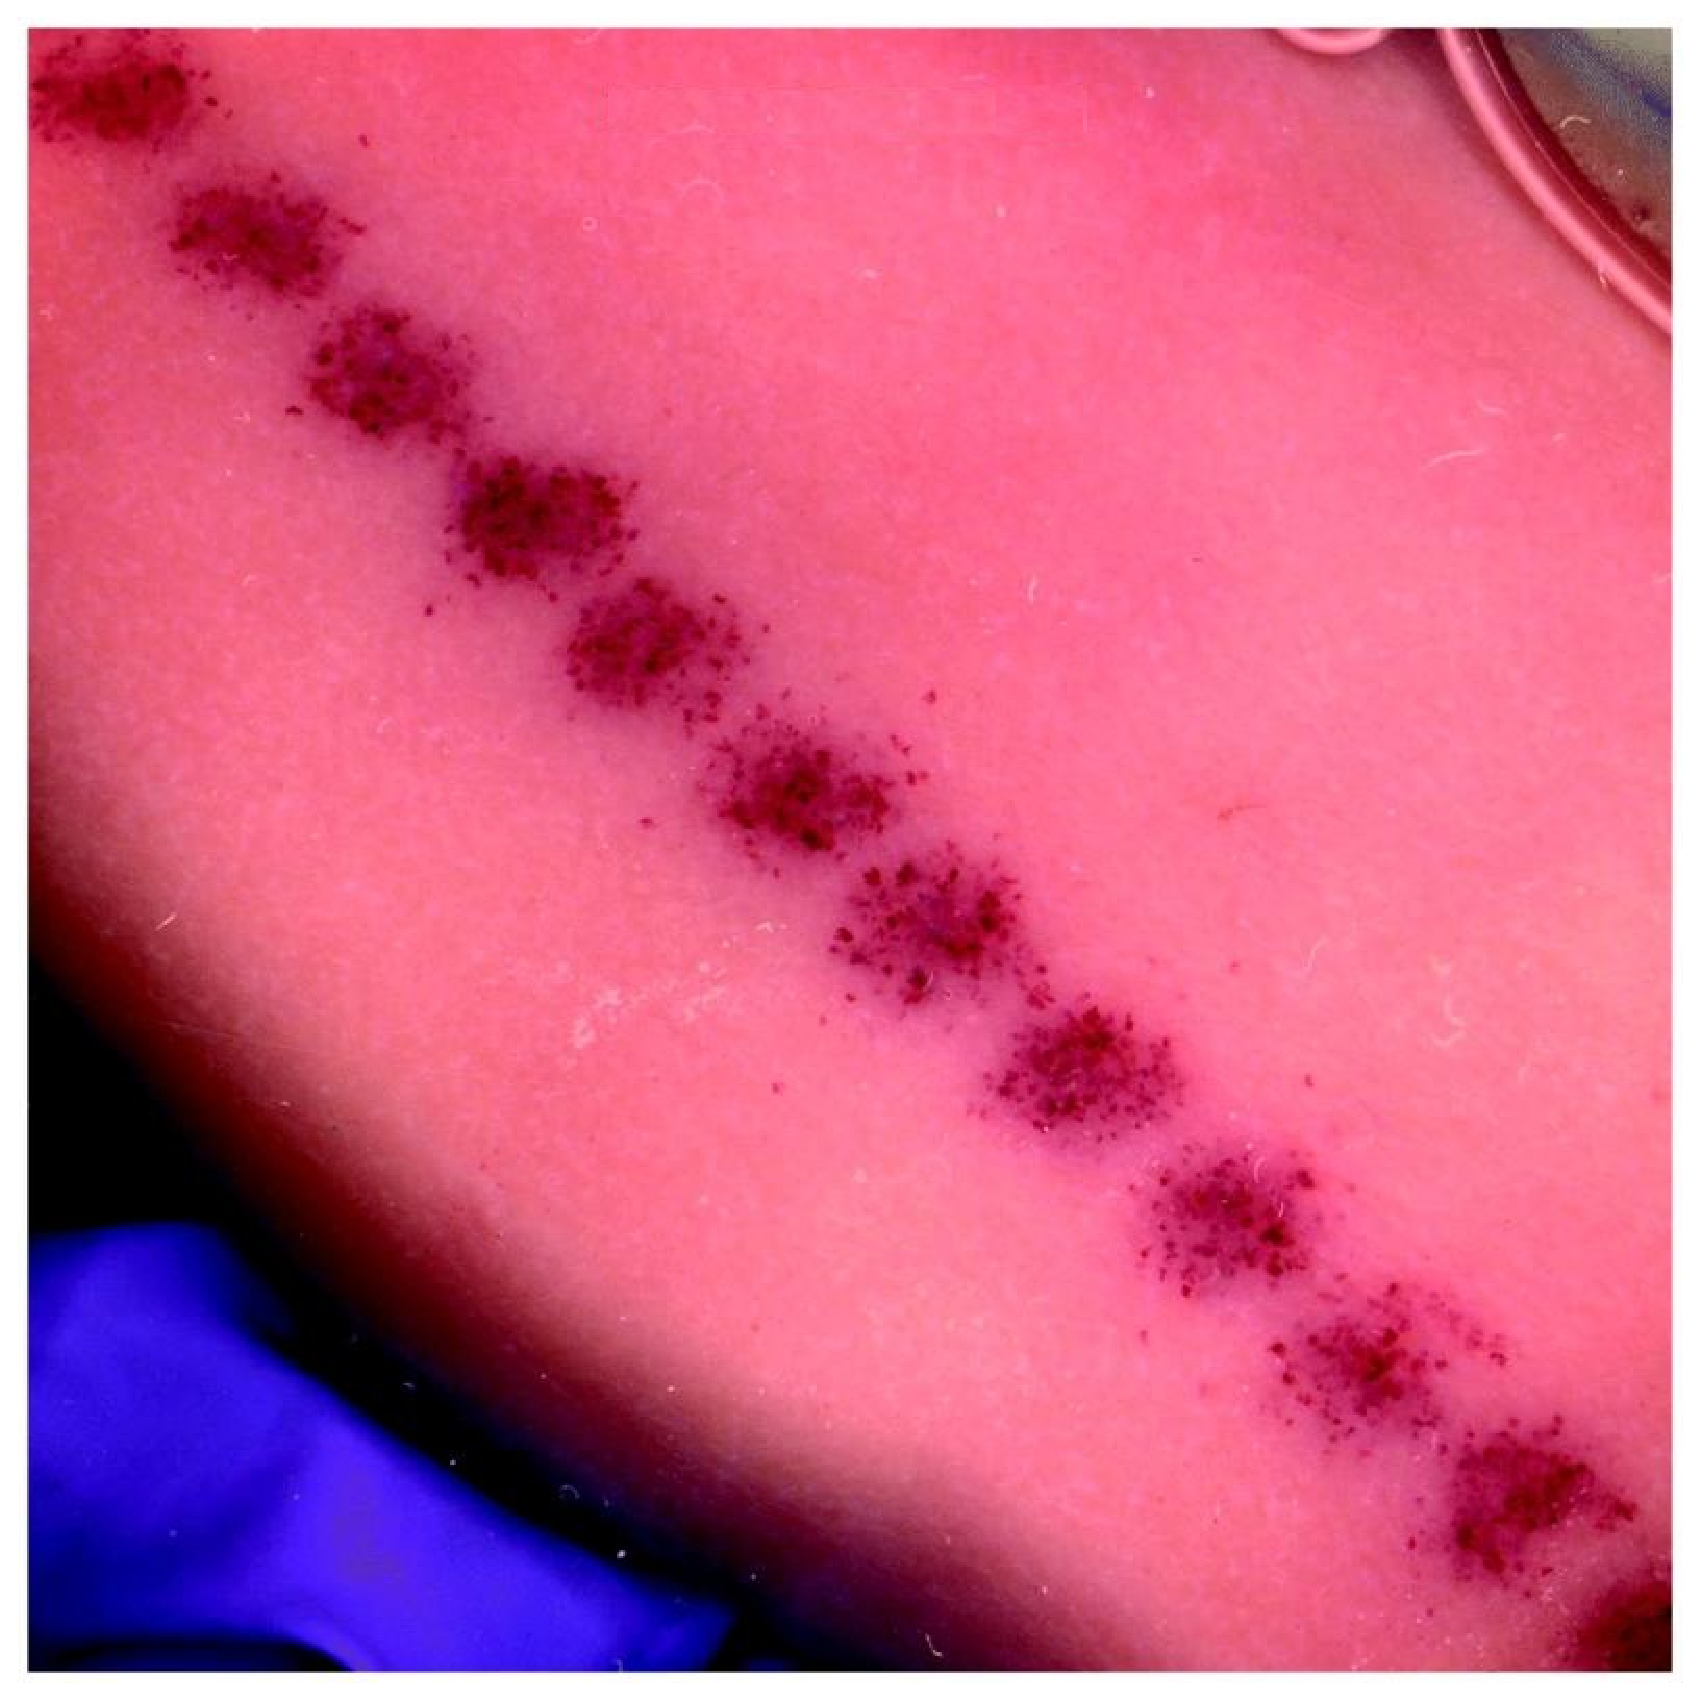
\includegraphics[height=0.25\textheight]{./figs/Kidney_Bleed}\hfill
      };%
      \begin{scope}[x={(image.south east)},y={(image.north west)}]%
        \node[font=\tiny,right] at (0.01,0.03) {\scalebox{0.4}{\textcolor{white}{Courtesy of D. L. Miller}}};%
      \end{scope}%  
    \end{tikzpicture}\hfill%
    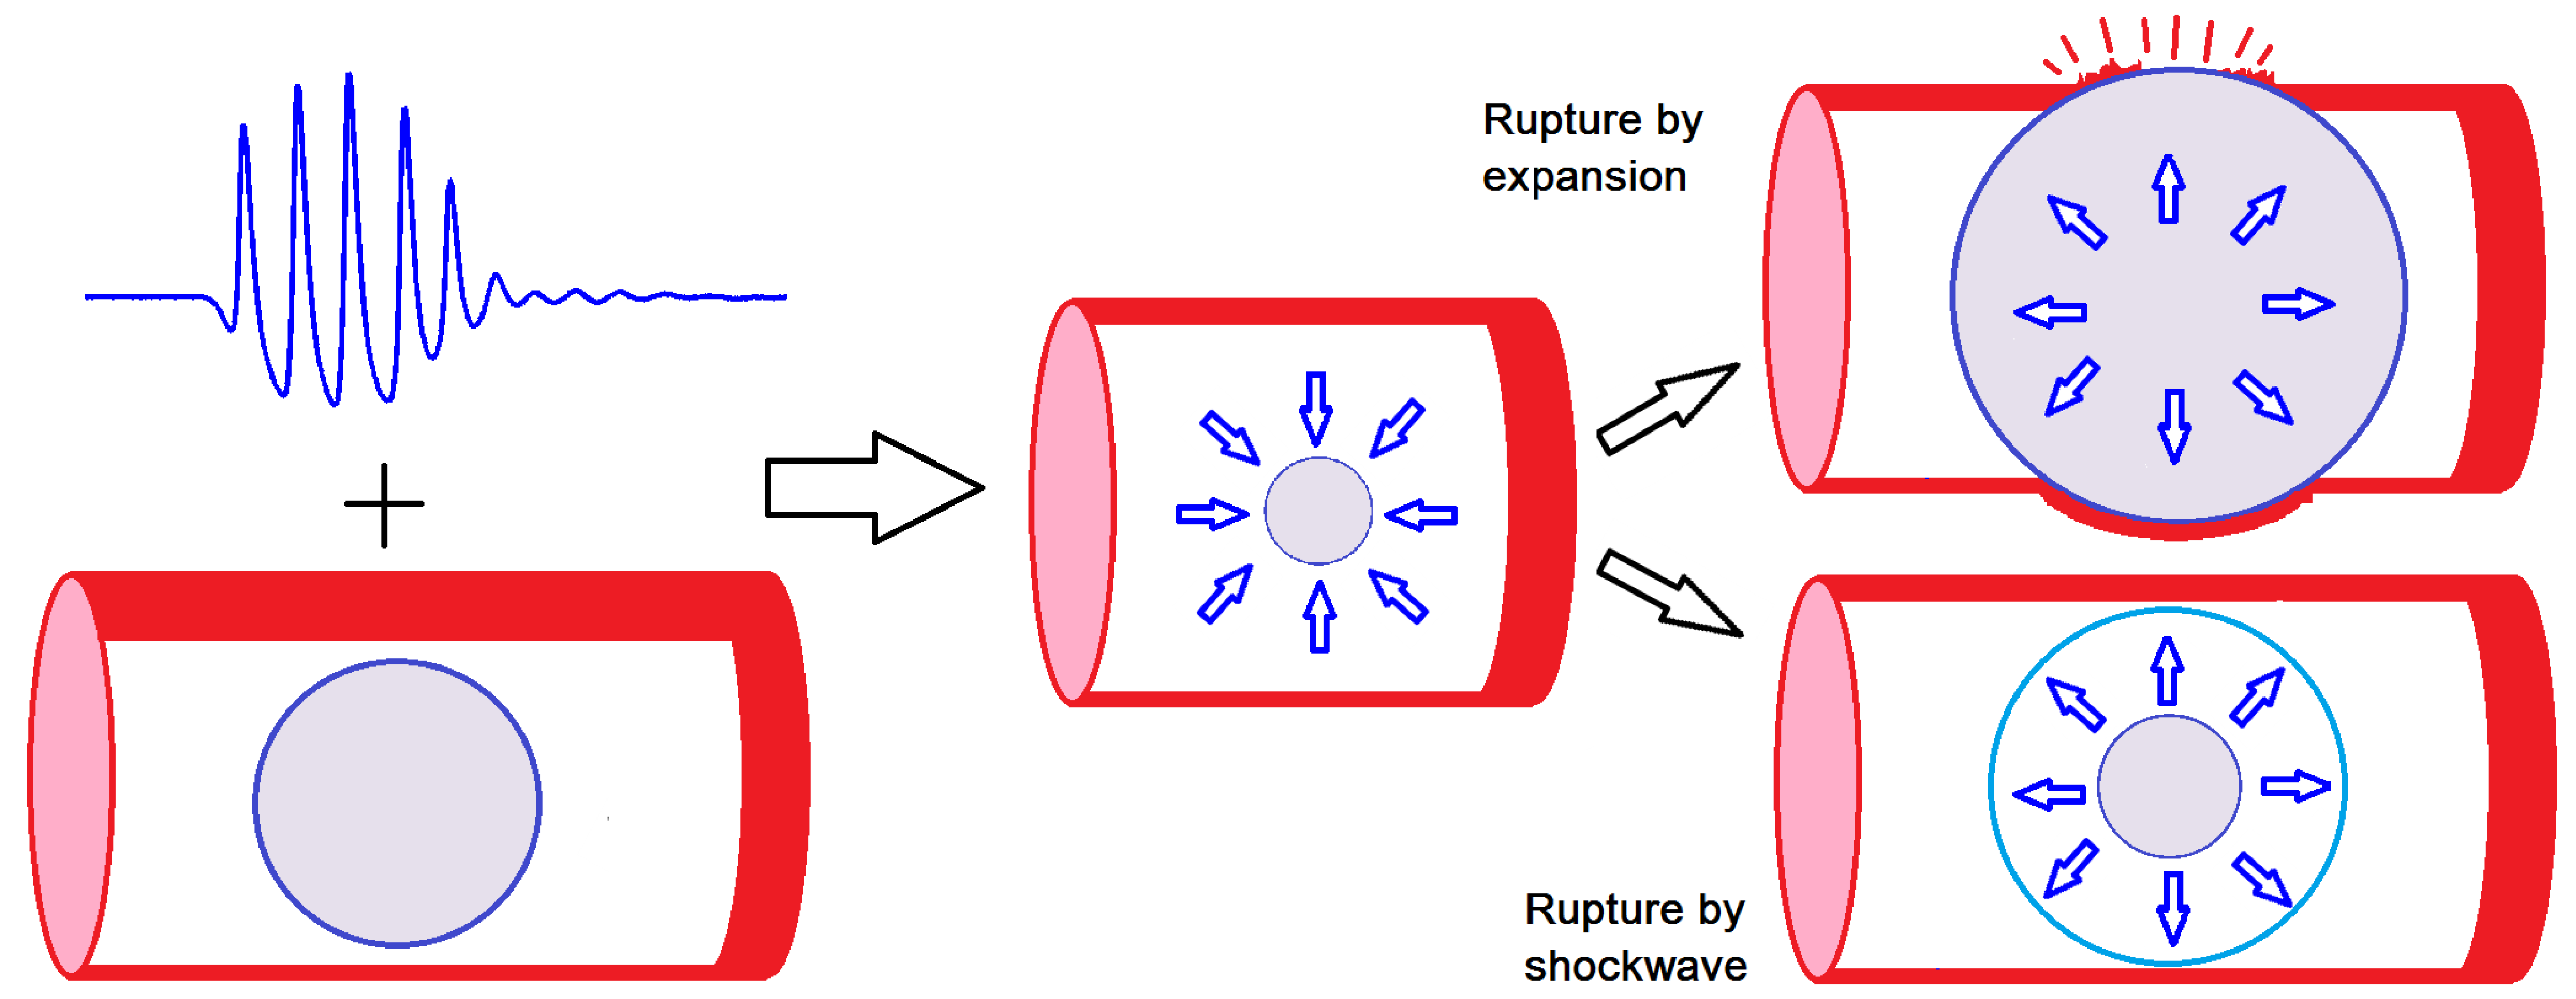
\includegraphics[height=0.25\textheight]{./figs/cavitation_hemorrhage}
  \end{figure}
  {\small
    \begin{itemize}
    \item Diagnostic Ultrasound (DUS) is ubiquitous and generally very safe.
    \item CEUS uses echogenic microbubbles for contrast, but these may act as cavitation nuclei and can lead to hemorrhage.
    \item Lung Hemorrhage (LH) is the only known bioeffect of non-contrast diagnostic ultrasound under clinically safe conditions.
    \end{itemize}
  }
\end{frame}
%% 
%% 
\begin{frame} \frametitle{\textit{Past work}: Theoretical microbubble dynamics in a viscoelastic medium at capillary breaching thresholds}
  \vspace*{\fill}
  \begin{minipage}{\textwidth}
    \begin{minipage}{0.3\textwidth}
      \begin{figure}
        \centering
            \begin{tikzpicture}
      \node[anchor=south west,inner sep=0] (image) at (0,0) {
        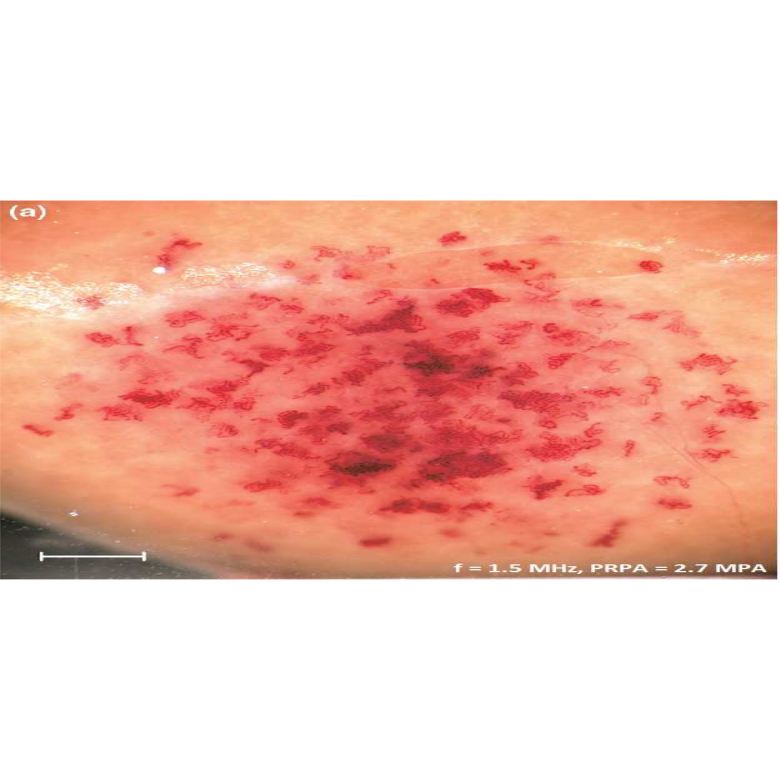
\includegraphics[width=0.8\textwidth]{./figs/Kidney_Bleed3}\hfill
      };%
      \begin{scope}[x={(image.south east)},y={(image.north west)}]%
        \node[font=\tiny,right] at (0.01,0.03) {\scalebox{0.4}{\textcolor{white}{\cite{Miller2008b}}}};%
      \end{scope}%  
    \end{tikzpicture}\hfill%
        
      \end{figure}
    \end{minipage}
    \begin{minipage}{0.68\linewidth}
      {\tiny
        \scalebox{0.9}{$
          \left(1-\frac{\dot{R}}{C}\right) R \ddot{R} + \frac{3}{2}\left(1-\frac{\dot{R}}{3 C}\right) \dot{R}^2 = \left(1+\frac{\dot{R}}{C}\right) \left[p_B- 1 -p_a -
            \frac{R}{C}\frac{dp_a}{dt}\right] +\frac{R}{C} \dot{p}_B,$\\}%
        \vspace*{2pt}
        \scalebox{0.9}{$p_B = \left(1+\frac{2}{We}\right)\frac{1}{R^{3\gamma}}-\frac{2}{WeR} + \tau_R,$\\}

        \vspace*{0.5cm}
        \begin{tabular}{l l c l}
          Parameter & Dimensional value & & Dimensionless number \\ \hline
          Viscosity & $\mu=0.015$ (Pa s) & $\mapsto$ & $Re=\rho u R_o / \mu = 2/3$ \\
          Elasticity & $G=10^5$ (Pa) & $\mapsto$ & $Ca= \rho u^2 / G = 1.0$ 	\\
          Surface tension & $S=0.056$ (N/m) & $\mapsto$ & $We=\rho u^2 R_o / S$ = 2 \\
          Sound speed & $c=1570$ (m/s) & $\mapsto$ & $C = c/u=157$ \\  
          % Relaxation time & $\lambda = 0.5$ ($\mu$ s) & $\mapsto$ &	$De=\lambda u / R_o =0$ \\
        \end{tabular} 
      }
    \end{minipage}
  \end{minipage}

  \vfill

  \begin{minipage}{\textwidth}
    \includegraphics[width=0.6\textwidth]{../figs/bubble_figs/rt_nonlinear}\hfill
    \includegraphics[width=0.33\textwidth]{../figs/bubble_figs/rstarmax_f}  
  \end{minipage}
  \vfill
  \scalebox{0.7}{
    {\tiny Patterson, B., Miller, D. L., \& Johnsen, E. (2012). Theoretical microbubble dynamics in a viscoelastic medium at capillary breaching thresholds. JASA, 132(6), 3770.}
  }
\end{frame}
%% 
%% 
\begin{frame}
  \centering
  \begin{center}
    {\LARGE Part II: Current Project}\\
    
    Diagnostic ultrasound-induced lung hemorrhage and acoustic wave
    interactions with liquid-gas interfaces
  \end{center}
\end{frame}
%% 
%% 
\begin{frame} \frametitle{\vspace*{0.5cm}DUS-induced lung hemorrhage is not a new problem}
  {\small%
    \begin{itemize}%
    \item Lung Hemorrhage (LH) is the only known bioeffect of non-contrast DUS%
    \item Has been shown to occur in mice, rats, pigs, rabbits, monkeys \citep{Child1990,OBrien1997a,Tarantal1994a}.%
    \item DUS-induced LH does not appear to be a result of cavitation or heating.%
    \item The underlying physical damage mechanism is not understood.%
    \end{itemize}%
    % 
    \begin{figure}%
      \centering%
      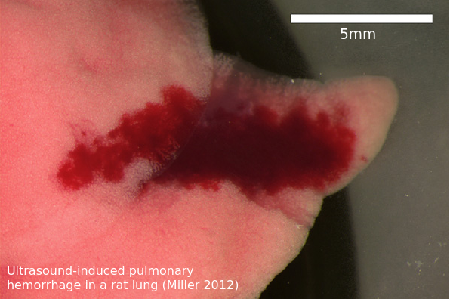
\includegraphics[width=0.5\textwidth]{LungBleed2} \nocite{Miller2012}%
    \end{figure}%
    % 
    \visible<2>{To gain insight into DUS-induced LH, we aim to use computational modeling and simulations to investigate DUS-lung interaction.}%
    % 
  }
\end{frame}
%% 
%% 
\begin{frame}\frametitle{\vspace*{0.5cm}We simulated and US-pulse impinging on a water-air interface}
  \begin{minipage}{0.62\textwidth}
    \begin{minipage}{\textwidth}
      \begin{figure}
        \centering
        \includegraphics[width=0.47\textwidth]{../figs/lung_figs/p0_vs_t_us}%
      \end{figure}
    \end{minipage}
  % 
    \begin{minipage}{\textwidth}
      \begin{figure}
        \centering \def\svgwidth{0.48\textwidth} {\footnotesize
          \import{../figs/lung_figs/}{usbe_lung_schematic3.pdf_tex}
          \hfill%
        }
        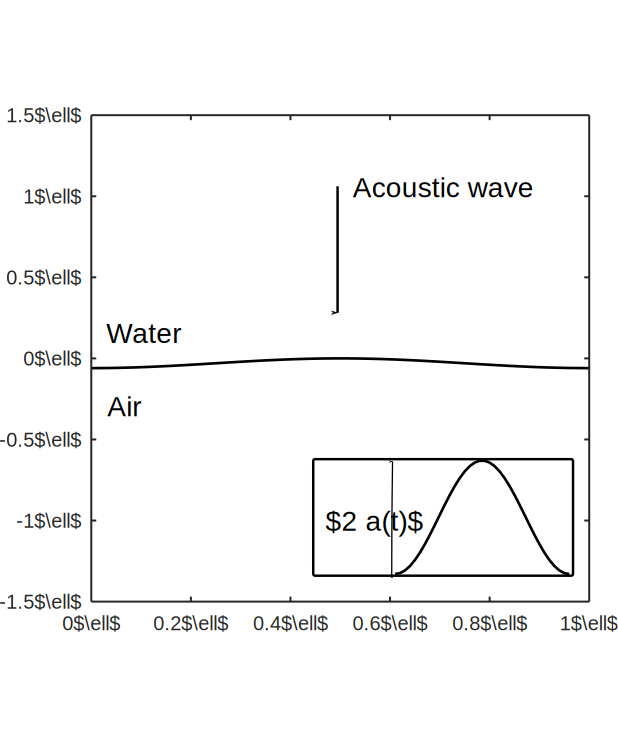
\includegraphics[width=0.48\textwidth]{../figs/lung_figs/usbe_model_schematic}
      \end{figure}
    \end{minipage}
  \end{minipage}
  % 
  \hfill
  %
  \begin{minipage}{0.36\textwidth}
    \movie[externalviewer]{\adjincludegraphics[trim={{0.32\width} 0 {0.32\width} 0 },clip=true,height = 0.7\textheight]{./figs/still.jpg}}{./figs/rmawave_1_10000000.0_0.03_45.0_0.0_1.0_1.0_100_100_blue.avi}
  \end{minipage}
  % 
\end{frame}
%%
%%
\begin{frame} \frametitle{\vspace*{0.5cm} Shock-driven fluid-fluid interfaces have been studied extensively}
  {\small
    \hfill%
    \begin{figure}
      \centering
      \begin{tikzpicture}%
        \node[anchor=south west,inner sep=0] (image) at (0,0) {
          \includegraphics[height=0.5\textheight]{../figs/lung_figs/baroclinic_schematic_vertical}%
        };%
        \begin{scope}[x={(image.south east)},y={(image.north west)}]%
          \node[font=\tiny,right] at (0.05,-0.05) {\textcolor{black}{Adapted from \cite{Heifetz2015}}};%
        \end{scope}%  
      \end{tikzpicture}%
      \hfill%
      \begin{tikzpicture}%
        \node[anchor=south west,inner sep=0] (image) at (0,0) {
          \def\svgwidth{0.6\textwidth}%
          \import{../figs/lung_figs/}{brouillette_fig3_mod_compact.pdf_tex}\hfill%
        };%
        \begin{scope}[x={(image.south east)},y={(image.north west)}]%
          \node[font=\tiny,right] at (0.15,-0.05) {\textcolor{black}{Adapted from \cite{Brouillette2002}}};%
        \end{scope}%  
      \end{tikzpicture}%
    \end{figure}
    \hfill
    \begin{itemize}
    \item Shocks deposit baroclinic vorticity at perturbed fluid-fluid interfaces \citep{Drake2006}, which drives the interface perturbation to grow.
    \item This is the Richtymyer-Meshkov ``instability''.
    \item This problem is not well studied for acoustic waves.
    \end{itemize}
  }  
\end{frame}
%% 
%% 
\begin{frame} \frametitle{We hypothesize that US waves generate baroclinic vorticity at air-tissue interfaces in the lungs, straining fragile alveolar walls.}%
  The vorticity generation equation\vspace{2pt}
  \only<1>{
    \scalebox{1.0}{$
      \frac{\partial \boldsymbol{\omega}}{\partial t}%
      +\left(\boldsymbol{u}\cdot\nabla\right)\boldsymbol{\omega}=% 
      \left(\boldsymbol{\omega}\cdot\nabla\right)\boldsymbol{u}%
      -\boldsymbol{\omega}\left(\nabla\cdot\boldsymbol{u}\right)%
      +\frac{\nabla\rho\times\nabla p}{\rho^2}%
      -\nabla\times\left(\frac{\nabla\cdot\boldsymbol{\tau}}{\rho}\right)%
      +\nabla\times\boldsymbol{B}%
      $%
    }
  }
  \only<2->{
    \scalebox{0.94}{$
      \frac{\partial \boldsymbol{\omega}}{\partial t}%
      +\left(\boldsymbol{u}\cdot\nabla\right)\boldsymbol{\omega}=% 
      \cancelto{0}{\left(\boldsymbol{\omega}\cdot\nabla\right)\boldsymbol{u}}%
      -\boldsymbol{\omega}\left(\nabla\cdot\boldsymbol{u}\right)%
      +\frac{\nabla\rho\times\nabla p}{\rho^2}%
      -\cancelto{0}{\nabla\times\left(\frac{\nabla\cdot\boldsymbol{\tau}}{\rho}\right)}%
      +\cancelto{0}{\nabla\times\boldsymbol{B}}%
      $
    }
  }
  \vfill 
  \begin{minipage}{\textwidth}
    \begin{minipage}{0.5\textwidth}
      {\footnotesize
        \begin{itemize}%
        \item Alveolar air-tissue interfaces have sharp density gradients%
          \vspace*{6pt}%
        \item US has strong pressure gradients%
          \vspace*{6pt}%
        \item US-induced baroclinic vorticity may cause strain, similar to shock-driven interfaces%
          \vspace*{6pt}%
        \item Linear acoustics does not capture this.
        \end{itemize}
      }
    \end{minipage}
    \begin{minipage}{0.5\textwidth}
      \begin{figure}
        \centering
        \begin{tikzpicture}%
          \node[anchor=south west,inner sep=0] (image) at (0,0) {%
            \def\svgwidth{\textwidth}
            {\footnotesize
              \import{../figs/lung_figs/}{usbe_lung_schematic2.pdf_tex} \hfill%
            }  
          };%
          \begin{scope}[x={(image.south east)},y={(image.north west)}]%
            \node[font=\footnotesize,right] at (0.6,0.72){ $\nabla p$};%
            \node[font=\footnotesize,right] at (0.59,0.515){ $\nabla \rho$};%
            \node[font=\tiny,right] at (0.7,0.05){\textcolor{gray}{wikimedia.org}};%
          \end{scope}%  
        \end{tikzpicture}%
      \end{figure}
    \end{minipage}
  \end{minipage}
\end{frame}
%% 
%% 
\begin{frame} \frametitle{Problem setup: We model the ultrasound-alveolar interaction as a 2D, compressible, inviscid fluid system.}
  \begin{figure}
    \centering
    \def\svgwidth{0.48\textwidth}
    {\footnotesize
      \import{../figs/lung_figs/}{usbe_lung_schematic2.pdf_tex} \hfill%
    }
    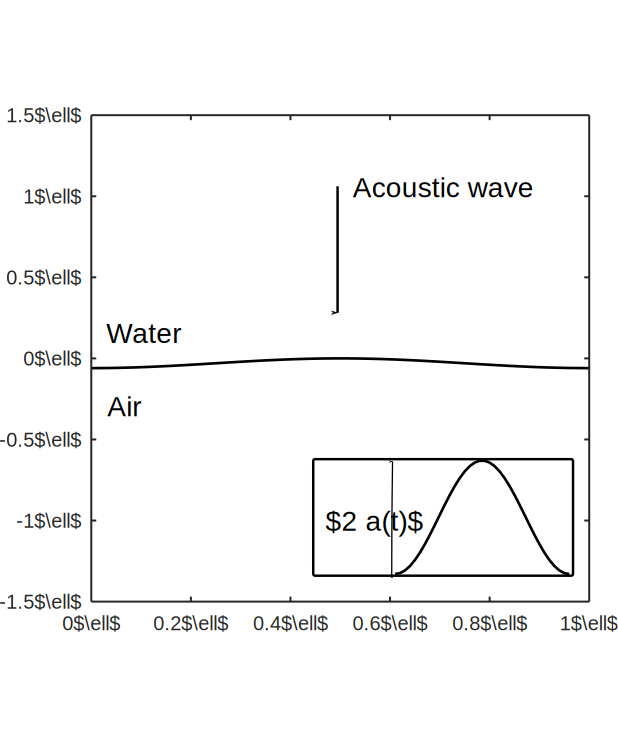
\includegraphics[width=0.48\textwidth]{../figs/lung_figs/usbe_model_schematic} \hfill
  \end{figure}
  An acoustic wave impinges downward from water toward a perturbed air interface $(a_0\equals0.03\lambda)$.
\end{frame}
%% 
%% 
\begin{frame} \frametitle{Trapezoidal and US pulse acoustic waveforms are used.}
  \begin{figure}
    \centering
    \visible<1-2>{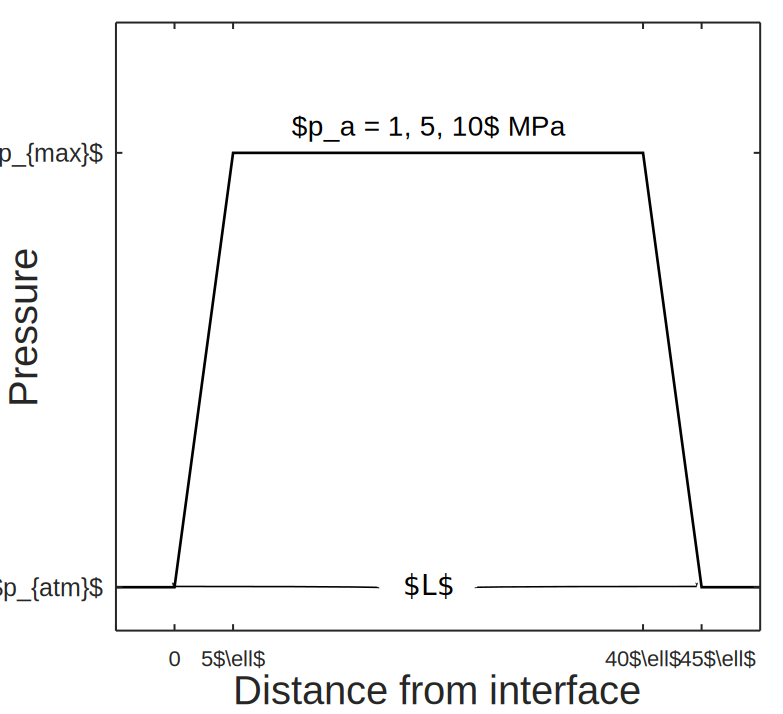
\includegraphics[width=0.47\textwidth]{../figs/lung_figs/p0_vs_y}}%
    \hfill%
    \visible<1>{\includegraphics[width=0.47\textwidth]{../figs/lung_figs/p0_vs_t_us}}%
  \end{figure}
  \begin{itemize}
  \item The trapezoidal waves is simple for understanding physics and analysis, but able to capture feature of US pulse.
  \item Pulse waveforms are used to check relevance to DUS.
  \end{itemize}
\end{frame}
%% 
%% 
\begin{frame} \frametitle{\vspace*{0.5cm}Governing Equations}
  \vfil\vspace*{0.5cm}
  {\small
    \hspace*{1cm}Euler equations of fluid motion
  }
  {\scriptsize
    \begin{align*}% 
      \frac{\partial \rho}{\partial t} + \frac{\partial \left(\rho u\right)}{\partial x} + \frac{\partial \left(\rho v\right)}{\partial y} = 0,\\
      \frac{\partial \rho u}{\partial t} + \frac{\partial}{\partial x}\left( \rho u^2+p\right)  + \frac{\partial}{\partial y}\left( \rho uv\right) = 0,\\
      \frac{\partial \rho v}{\partial t} + \frac{\partial}{\partial x}\left( \rho uv\right)  + \frac{\partial}{\partial y}\left( \rho v^2+p\right) = 0,\\
      \frac{\partial E}{\partial t} + \frac{\partial}{\partial x}\left[u\left(E+p\right)\right] + \frac{\partial}{\partial y}\left[v\left(E+p\right)\right] = 0,
    \end{align*}%
  }
  \vfil
  {\small
    \hspace*{1cm}Stiffened equation of state
  }
  {\scriptsize
    \begin{align*} \label{eq:stiffened_eos}%
      E=\frac{\rho\left(u^2+v^2\right)}{2} + \frac{p+\gamma B}{\gamma-1}.
    \end{align*}
  }
  \vfil
  {\small
    \hspace*{1cm}Advection equations for $\gamma,\,B$ prevent interface pressure oscillations.
  }
  \scriptsize{
    \begin{align*}
      \frac{\partial}{\partial t}\left(\frac{\gamma B}{\gamma-1}\right)%
      +u\frac{\partial}{\partial x}\left(\frac{\gamma B}{\gamma-1}\right)%
      +v\frac{\partial}{\partial y}\left(\frac{\gamma B}{\gamma-1}\right)%
      = 0,\\%
      %
      \frac{\partial}{\partial t}\left(\frac{1}{\gamma-1}\right)%
      +u\frac{\partial}{\partial x}\left(\frac{1}{\gamma-1}\right)%
      +v\frac{\partial}{\partial y}\left(\frac{1}{\gamma-1}\right)= 0%
    \end{align*}
  }
\end{frame}
%% 
%% 
\begin{frame} \frametitle{A high-order accurate computational solution strategy is invoked}
  \begin{minipage}{0.62\textwidth}
    \begin{itemize}
    \item An in-house developed code is used to solve the Euler equations.
    \item Numerical methods
      \begin{itemize}
      \item $3^{rd}$ order Discontinuous Galerkin method is used in space
      \item $4^{th}$ order Runge-Kutta time marching
      \item Roe Solver used to handle discontinuities
      \end{itemize}
    \item Acoustic waves are prescribed within the domain.
    \item Grid stretching reduces reflections.
    \item Grid size: $\lambda \times 70\lambda \, (L_x \times L_y)$
    \end{itemize}
  \end{minipage}
  \hfill%
  \begin{minipage}{0.34\textwidth}
    \begin{figure}
      \centering
      \def\svgwidth{\textwidth}
      {\footnotesize
        \import{../figs/lung_figs/}{domain_bcs.pdf_tex}%
      }
    \end{figure}
  \end{minipage}

\end{frame}
%% 
%% 
\begin{frame} \frametitle{\vspace*{0.5cm}Results: Evolution of the interface after 10 MPa trapezoidal wave}
  \begin{figure}
    \centering
    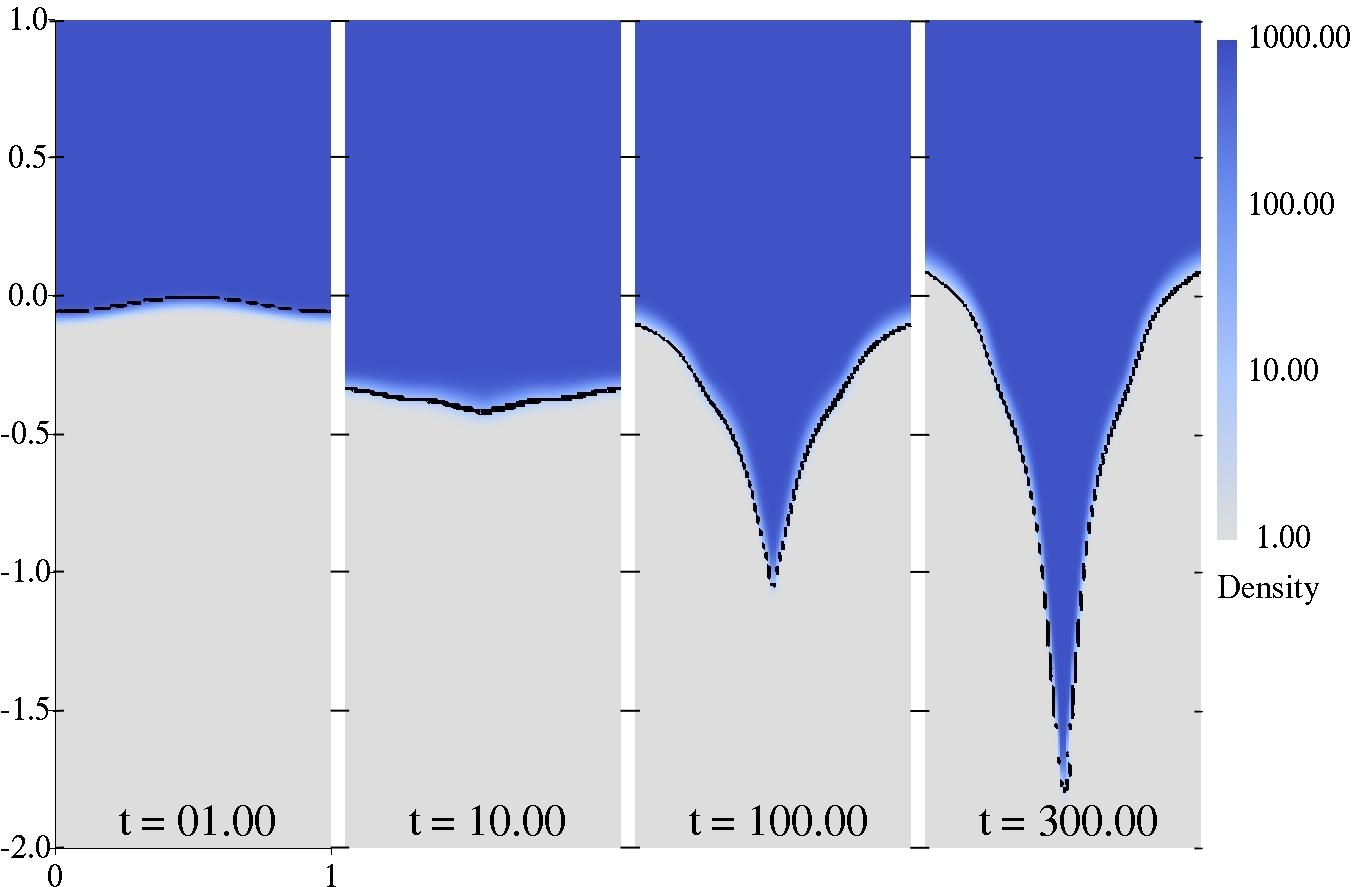
\includegraphics[width=0.85\textwidth]{../figs/lung_figs/snapshots_density_t1}
  \end{figure}
  {\small
    The interface perturbation evolves from a smooth sinusoid into a sharp point.
  }
\end{frame}
%% 
%% 
\begin{frame} \frametitle{\vspace*{0.5cm}Results: Evolution of the interface}
  \begin{figure}
    \hfill%
    \centering
    \includegraphics[height=0.5\textheight]{../figs/lung_figs/trapz10_intf_schematic}%
    \hfill%
    % 
    \begin{tikzpicture}%
      \node[anchor=south west,inner sep=0] (image) at (0,0) {%
        \includegraphics[height=0.5\textheight]{../figs/lung_figs/p0_vs_t_nd.pdf}%
      };%  
      \begin{scope}[x={(image.south east)},y={(image.north west)}]%
        \node[font=\footnotesize,right] at (0.22,0.18){ $t_1$};%
        \node[font=\footnotesize,right] at (0.22,0.8){ $t_2$};%
        \node[font=\footnotesize,right] at (0.83,0.8){ $t_3$};%
        \node[font=\footnotesize,right] at (0.82,0.18){ $t_4$};%
      \end{scope}%  
    \end{tikzpicture}%
    \hfill%
    % 
  \end{figure}
  The interface perturbation is initially compressed $(0^+\leq t\leq5)$, experiences a phase change $(t=5)$, then grows $t>5$.
\end{frame}
%% 
%% 
\begin{frame} \frametitle{\vspace*{0.5cm}Results: Late-time evolution of the interface}
  \begin{figure}
    \centering%
    \begin{tikzpicture}%
      \node[anchor=south west,inner sep=0] (image) at (0,0) {%
        \includegraphics[width=0.6\textwidth]{../figs/lung_figs/interface_multi-amp_loglog_roe_t1000_nolines}%
      };%
      \begin{scope}[x={(image.south east)},y={(image.north west)}]%
        \node[font=\footnotesize,right] at (0.4,0.7){ $10$ MPa};%
        \node[font=\footnotesize,right] at (0.6,0.4){ $5$ MPa};%
      \end{scope}%  
    \end{tikzpicture}%
  \end{figure}
  \begin{center}
    We suspect vorticity is driving this late time growth.
  \end{center}
\end{frame}
%% 
%% 
\begin{frame} \frametitle{\vspace*{0.5cm}Results: Vorticity dynamics}
  \begin{figure}
    \centering
    \includegraphics[width=0.8\textwidth]{../figs/lung_figs/snapshots_vorticity_t1}
  \end{figure}
  % 
  Vorticity is initially deposited in the air-dominated portion of the
  interface region. As the interface evolves, some vorticity advects
  with it.
  \note{A linear scale that changes each timestep is used for visual reasons.}
\end{frame}
%% 
%% 
\begin{frame} \frametitle{\vspace*{0.5cm}Results: A closer look at how circulation is deposited.}
  \begin{figure}
    \centering
    \hfill%
    \includegraphics[width=0.48\textwidth]{../figs/lung_figs/trapz10_circ_schematic}
    \hfill%
    % 
    \begin{tikzpicture}%
      \node[anchor=south west,inner sep=0] (image) at (0,0) {%
        \includegraphics[height=0.5\textheight]{../figs/lung_figs/p0_vs_t_nd.pdf}%
      };%  
      \begin{scope}[x={(image.south east)},y={(image.north west)}]%
        \node[font=\footnotesize,right] at (0.22,0.18){ $t_1$};%
        \node[font=\footnotesize,right] at (0.22,0.8){ $t_2$};%
        \node[font=\footnotesize,right] at (0.83,0.8){ $t_3$};%
        \node[font=\footnotesize,right] at (0.82,0.18){ $t_4$};%
      \end{scope}%  
    \end{tikzpicture}%
    \hfill%
  \end{figure}
  Both the compression and expansion deposit vorticity.
  \note{ To Do: Label phase-inversion.
    Mauro's Questions:\\
    (1) What is the vorticity doing during the phase inversion?
  }

\end{frame}
%% 
%% 
\begin{frame} \frametitle{\vspace*{0.5cm}Results: Late-time evolution of the interface}
  \begin{figure}
    \centering%
    \begin{tikzpicture}%
      \node[anchor=south west,inner sep=0] (image) at (0,0) {%
        \includegraphics[width=0.48\textwidth]{../figs/lung_figs/interface_multi-amp_loglog_roe_t1000}%
      };%
      \begin{scope}[x={(image.south east)},y={(image.north west)}]%
        \node[font=\footnotesize,right] at (0.38,0.7){ $10$ MPa};%
        \node[font=\footnotesize,right] at (0.57,0.4){ $5$ MPa};%
      \end{scope}%  
    \end{tikzpicture}%
    \hfill%
    \includegraphics[width=0.48\textwidth]{../figs/lung_figs/circulation_multi-amp_roe_t1000}%
  \end{figure}
  {\small
    From dimensional analysis, we expect a purely circulation driven interface to grow as $a(t) \sim \sqrt{\Gamma t}.$
  }

\end{frame}
%%
%%

\begin{frame}\frametitle{ \vspace*{0.5cm} Results: Dependence on the length of the wave}
  \begin{figure}
    \centering
    \includegraphics[width=0.48\textwidth]{../figs/lung_figs/interface_multi-lag}
    \includegraphics[width=0.48\textwidth]{../figs/lung_figs/circulation_multi-lag_fixed}
  \end{figure}
  The length of the wave strongly effects the vorticity deposited and
  thus the long-term dynamics of the interface.
  %
  \note{ To Do: Remove
    un-neccessary lines, $15\lambda$,
    Mauro's Questions:\\
    (1) Is there a way to non-dimensionalize this show that the
    transition of the physics occurs between $L = 20 - 30 \lambda$.
    (1A): This essentially boils down to figuring out the speed of the
    interface evolution and modeling the time at which the
    phase-inversion will occur.\\Maybe I should subtract
    $\Delta L_{lag}$ to see this better, or divide $\gamma$ by
    $a(t=t_{phase-reversal})^n$ or $\Delta L_{Lag}^n$.\\
    (2) What is the Reynolds number?
  }
\end{frame}
%% 
%% 
\begin{frame} \frametitle{\vspace*{0.5cm}Order of magnitude analysis of vorticity generation}%
  \vspace*{-0.25cm}
  \scriptsize{
    \begin{align*}
      \frac{\partial \vec{\omega}}{\partial t}+\left(\vec{u}\cdot\nabla\right)\vec{\omega} =% 
      - \vec{\omega}\left(\nabla\cdot\vec{u}\right) + \frac{\nabla\rho\times\nabla p}{\rho^2}.%
    \end{align*}

    \visible<2->{
      \text{Acoustic Relations and operator treatments}%
      \begin{align*}
        \Delta p_a=\pm\Delta u_a \rho c=c^2\Delta \rho_a, \quad\qquad \norm{\nabla f} \sim \norm{\nabla\cdot f} \sim \norm{\nabla\times f}= \orderof{\left|\Delta f\right|/\Delta L}%
      \end{align*}
    }
    \visible<3->{
      Baroclinic vorticity generation%
      \begin{align*}
        \norm{\frac{\nabla\rho\times\nabla p}{\rho^2}} = \orderof{\frac{\abs{\Delta \rho_I}}{\abs{\Delta L_I}}\frac{\abs{\Delta p_a}}{\abs{\Delta L_a}}\frac{1}{\abs{\rho}^2}\abs{\theta}}
      \end{align*}
    }
    
    \visible<4->{
      Advective and compressible vorticity generation - $\norm{\vec{\omega}} = \int_0^{\Delta t_a} (\text{baroclinic term}) dt$
      \begin{align*}
        \norm{\left(\vec{u}\cdot\nabla\right)\vec{\omega}} \sim \norm{-\vec{\omega}\left(\nabla\cdot\vec{u}\right)} = \orderof{\left[\frac{\abs{\Delta u_a}}{\abs{\Delta L_a}}\right]^2},
      \end{align*}
    }

    \visible<5->{
      Comparing terms for our our problem
      \begin{align*}
        \Delta t_a\approx5\lambda/c_{w}, \qquad \Delta L_a=5\lambda, \qquad \Delta p_a = 10 MPa, \qquad \Delta L_I \approx 0.05\lambda\\%
        \frac{\norm{\frac{\nabla\rho\times\nabla p}{\rho^2}}}{\norm{-\vec{\omega}\left(\nabla\cdot\vec{u}\right)}} = \frac{c}{\abs{\Delta u_a}} = \frac{\rho}{\abs{\Delta \rho_a}}=\orderof{10^2}%
      \end{align*}
    }
    \visible<6->{
      Calculated values at $t=1$: 
      \begin{center}
        $\frac{\nabla\rho\times\nabla p}{\rho^2}=7.7\,\text{e}{-3},\qquad$
        $\left(\vec{u}\cdot\nabla\right)\vec{\omega}=-5.3\text{e}{-5},\qquad$%
        $-\vec{\omega}\left(\nabla\cdot\vec{u}\right)=2.7\text{e}{-5},\qquad$%
      \end{center}
    }
  }
\end{frame}
%% 
%% 
\begin{frame} \frametitle{\vspace*{0.5cm}Vorticity generation occurs predominately in gas-dominated fluid}
  \vspace*{-.5cm}
  {\scriptsize
    \begin{figure}
      \centering
      \hfill
      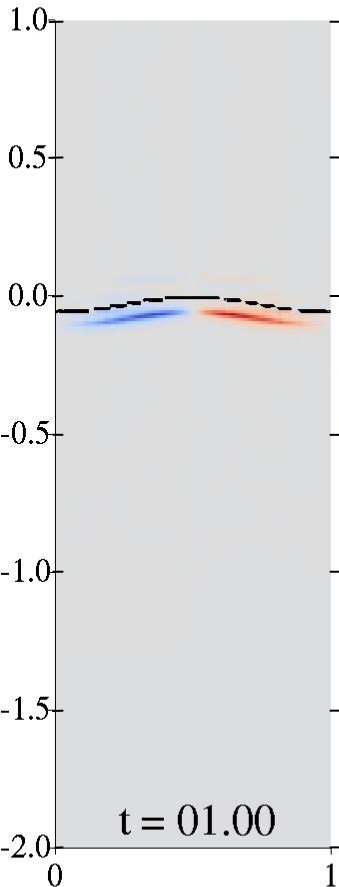
\includegraphics[width=.13\textwidth]{../figs/lung_figs/snapshots_vorticity_t1_only} \hfill
      \includegraphics[width=.38\textwidth]{./figs/vorticity_vs_y0} \hfill
      \includegraphics[width=.38\textwidth]{./figs/circ_y0_dist}
      \hfill
    \end{figure}
    % 
    \vspace*{-.3cm}
    \begin{align*}%
      \frac{\norm{\frac{\nabla\rho\times\nabla p}{\rho^2}}_{air\quad}}{\norm{\frac{\nabla\rho\times\nabla p}{\rho^2}}_{water}}%
      =&\orderof{\abs{\boldsymbol{T}}\left(\frac{\abs{\rho^-}}{\abs{\rho^+}}\right)^2}%
         \approx 357
    \end{align*}
    \vspace*{-.25cm}
    % 
    \begin{itemize}
    \item 97\% of circulation appears in fluid with $y_0<0.5$
    \item Computed circulation ratio from air($y_0<0.1$) to water($y_0>0.9$) is $\approx 27$
    \end{itemize}
  }
\end{frame}
%% 
%% 
\begin{frame} \frametitle{\vspace*{0.5cm}Interface response to a 10 MPa US pulse}
  \begin{figure}
    \centering
    \includegraphics[width=0.48\textwidth]{../figs/lung_figs/us_intf_schematic}\hfill
    \includegraphics[width=0.48\textwidth]{../figs/lung_figs/us_circ_schematic}
  \end{figure}
  \begin{itemize}
  \item Qualitatively, the interface response for the 10 MPa US pulse looks very similar to the 10 MPa trapezoidal wave. 
  \item The circulation deposited is of the same order as the equivalent amplitude trapezoidal wave.
  \end{itemize}

\end{frame}
%%
%%
\begin{frame} \frametitle{\vspace*{0.5cm}Conclusions thus far}
  \begin{itemize}
  \item Acoustically-generated baroclinic vorticity is likely capable
    of significantly deforming perturbed liquid gas interfaces.\vfill%
  \item Baroclinic vorticity is predominantly deposited in gaseous fluids.\vfill%
  \item Changes in the acoustic waveform that have little effect on
    the interface during the wave-interface interaction can
    substantially effect the interface over long periods of time, via
    vorticity.\vfill%
  \item Interface response from an US wave is qualitatively similar to that for a trapezoidal wave.
  \end{itemize}
  \note{
    Mauro's Questions:\\
    (1) How important baroclinic vorticity relative to viscous and body forces?
  }
\end{frame}
%% 
%% 
\begin{frame}
  \centering
  \begin{center}
    \LARGE Part III: Future work
  \end{center}
\end{frame}
%% 
%% 
\begin{frame}\frametitle{\vspace*{0.5cm}I plan to increase the relevance to DUS}
  \begin{minipage}{0.5\textwidth}
    \begin{itemize}
      \alert<1>{
    \item Calculate interface strain\vfill%
    \vspace*{5pt}

    \item Calculate stress at the interface\vfill%
    \vspace*{5pt}
    }
    \alert<2>{
    \item Investigate the effects of alveolar side wall structures\vfill%
    }
    \vspace*{5pt}
    \alert<3>{
    \item Investigate the propagation of acoustic waves into
      subsequent layers of alveoli\vfill%
      }
    \end{itemize}
  \end{minipage}
  \begin{minipage}{0.49\textwidth}
    \only<1>{
    \def\svgwidth{\textwidth}%
    {\tiny
      % 
      \import{./figs/}{usbe_lung_model_arclength.pdf_tex}%
    }
  }
  \includegraphics<2>[width=\textwidth]{../figs/lung_figs/usbe_model_schematic_walls}
  \includegraphics<3>[width=\textwidth]{../figs/lung_figs/usbe_model_schematic_periodic}
  \end{minipage}
\note{Mauro's Question:
  (1) Would a bubble-like configuration be more relevant/useful?
  }
\end{frame}
%% 
%% 
\begin{frame}\frametitle{\vspace*{0.5cm}I aim to further our understanding of the relevant fluid mechanics}
  \begin{figure}
    \centering
    \includegraphics[height=0.4\textheight]{../figs/lung_figs/trapz10_intf_schematic}\hspace{1cm}%
    \includegraphics[height=0.4\textheight]{../figs/lung_figs/trapz10_circ_schematic}%
  \end{figure}

{\small
  \begin{itemize}
  \item Explain the discrepancies between numerical results and $a(t)\sim\sqrt{\Gamma t}$%
    \vspace*{5pt}
  \item Develop a model to approximate the circulation deposited on a
    slightly perturbed interface by a compression or expansion wave
    \vspace*{5pt}
  \item Develop a model to predict the interface phase-reversal time for a compression wave
    \vspace*{5pt}
  \item Design an acoustic waveform to minimize circulation deposited and interface growth.
    \vspace*{5pt}
  \item Investigate cause of late time circulation growth
  \end{itemize}
}
\end{frame}
%% 
%% 
%%%%%%%%%%%%%%%%%%%%%%%%%%%%%%%%%%%%%%%%%%%%%%%%%%%%%%%%%%%%%%%%%%%%%% 


\section{Citations}
\bibliographystyle{../tex/myauthordate2}
% Give this command the relative path to the .bib file.
\bibliography{../../../literature/library}


%%%%%%%%%%%%%%%%%%%%%%%%%%%%% 

% \begin{frame} \vspace{\fill} \begin{center} \Huge 
%     Thanks a lot!\\ \vspace{\fill} Questions? 
%   \end{center} \vspace{\fill} \end{frame} 


\end{document}






% Template Created by Brandon Patterson - awesome@umich.edu
%%% Local Variables:
%%% mode: latex
%%% TeX-master: t
%%% End:
